\chapter{Proposed Work}

This project aims to develop a comprehensive system that integrates advanced machine learning techniques with CNN-based object detection models to improve pose detection accuracy in classical performing arts, specifically focusing on traditional forms like Kathakali. The process begins with the collection and meticulous curation of high-quality images, followed by detailed manual annotation to ensure a robust dataset. This dataset will serve as the foundation for training specialized models to recognize complex poses and culturally specific gestures, which are often challenging for conventional pose detection systems due to the presence of elaborate costumes and accessories. The system will undergo rigorous model development and training, leveraging annotated data to refine its accuracy in landmark and bounding box detection. Ultimately, our goal is to deploy this system as a tool for recognizing and preserving culturally significant art forms, enabling precise interpretation of gestures while contributing to pose detection research in unique, traditionally underrepresented areas.

\section{Data Collection}
The initial phase of our project has focused on the careful collection and curation of a high-quality dataset that will serve as the foundation for our pose detection model in classical performing arts. This stage involved sourcing images from diverse origins, including frame extractions from video recordings and still images of traditional performances. This comprehensive approach enabled us to amass a diverse and representative set of images showcasing various poses and gestures characteristic of the art form.

After gathering the initial pool of images, we meticulously filtered out unwanted photos, ensuring that only the most suitable and clear images were retained for further processing. This rigorous curation process resulted in a refined dataset comprising over 1,000 high-quality images, capturing the nuanced movements and expressions integral to the performance style.

\begin{table}[h]
\centering
\begin{tabular}{|l|l|}
\hline
\textbf{Attribute} & \textbf{Details} \\ \hline
Total Images & 1,346 \\ \hline
Bounding Boxes & 1,346 images \\ \hline
Landmark Annotations & 342 images \\ \hline
Annotation Tools Used & CVAT, MakeSense AI \\ \hline
Total Landmark Points Per Image & 14 \\ \hline
\end{tabular}
\caption{Dataset Overview}
\label{tab:dataset_overview}
\end{table}

Subsequent to collection, we undertook a detailed annotation process to enhance the dataset's usability for training purposes. Using tools such as CVAT and MakeSense AI, we focused on two main types of annotations:

\begin{enumerate}
    \item Bounding boxes: Each image was annotated with bounding boxes to delineate the performer's silhouette within the frame, thereby facilitating initial object detection tasks. 
    \item Landmark points: Approximately 200 images were further annotated with 14 landmark points, providing detailed positional data on key body points crucial for advanced pose detection. These landmarks include:
    \begin{itemize}
    \item Head
    \item Shoulders (left and right)
    \item Elbows (left and right)
    \item Wrists (left and right)
    \item Mid-torso/Neck
    \item Hips (left and right)
    \item Knees (left and right)
    \item Ankles (left and right)
    \end{itemize}
\end{enumerate}
This dual-layered annotation approach not only enriches the dataset but also optimizes it for future training stages, where CNN-based object detection models will be employed to develop the core of the pose detection system.

% \begin{figure}[h]
% \centering
% 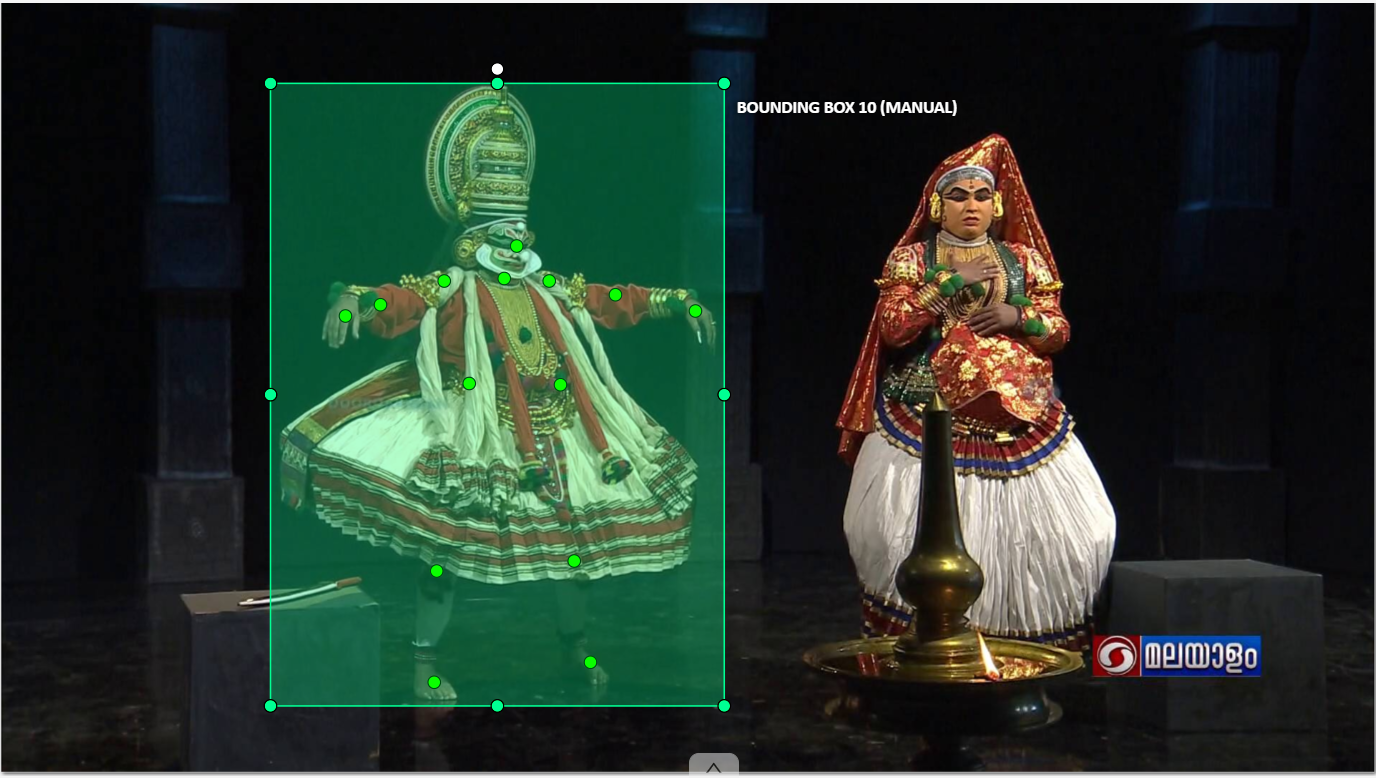
\includegraphics[width=\linewidth]{image.png}
% \caption{Annotated image from the dataset showcasing bounding boxes and key landmark points (head, shoulders, elbows, wrists, mid-torso/neck, hips, knees, and ankles). The detailed annotations highlight the precision in capturing critical body landmarks, essential for accurate pose detection in classical performing arts.}
% \end{figure}
\begin{figure}[h]
\centering
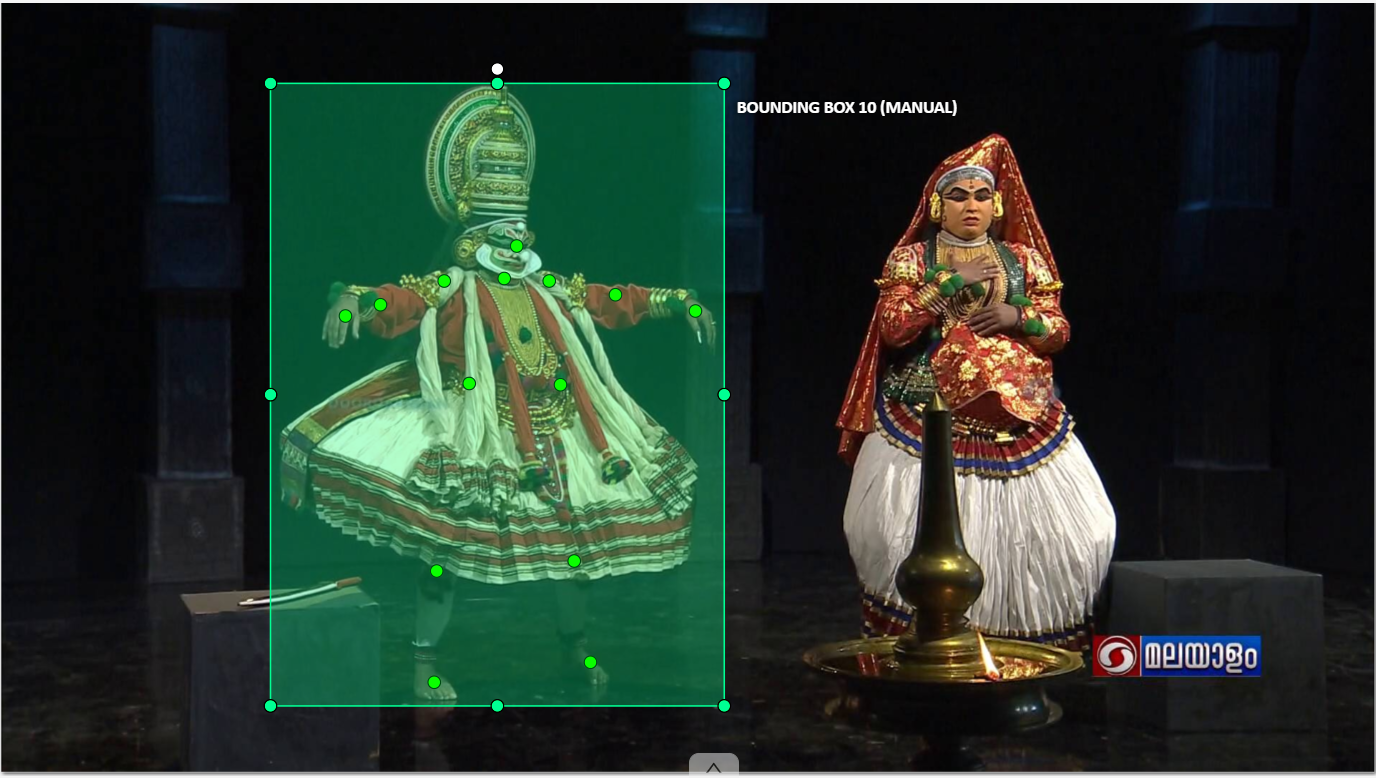
\includegraphics[width=\linewidth]{image.png}
\caption{Annotated image from the dataset showcasing bounding boxes and key landmark points (head, shoulders, elbows, wrists, mid-torso/neck, hips, knees, and ankles). The detailed annotations highlight the precision in capturing critical body landmarks, essential for accurate pose detection in classical performing arts. 
\textbf{\cite{youtube2024kathakali2}.}}
\end{figure}

The dataset structure and annotation process are detailed in Table \ref{tab:dataset_overview}, and a sample annotated image with both bounding boxes and landmark points is shown in Figure 3.1. This curated dataset is a crucial step forward, laying the groundwork for the accurate detection and analysis of complex poses in later stages of the project.

\begin{table}[h]
\centering
\resizebox{\textwidth}{!}{%
\begin{tabular}{|c|c|c|c|c|}
\hline
\textbf{Task} & \textbf{\# Images} & \textbf{Annotation} & \textbf{Vesham (Character)} & \textbf{Scope} \\ \hline
Person Detection & 1,346 & Bounding Box (B-box Coordinates) & Pacha & In the wild \\ \hline
Landmark Detection & 342 & 14 Key Points & Pacha & In the wild \\ \hline
\end{tabular}%
}
\caption{Dataset Overview}
\label{tab:dataset_overview}
\end{table}

Through these steps, we have created a robust and well-annotated dataset that will support the precise training and refinement of our model, ensuring it can effectively capture the distinctive poses and gestures specific to classical performing arts. This dataset will be instrumental in developing a system capable of recognizing and analyzing the unique and culturally specific movements characteristic of these traditional art forms.

\clearpage

\newgeometry{left=0.5cm, right=0cm}
\begin{table}[h]
\centering
\small
\begin{tabular}{|l|l|l|}
\hline
\textbf{Landmark} & \textbf{Description} & \textbf{Relevance for Pose Detection} \\ \hline
Head & Topmost part of the body & Detects orientation and gesture \\ \hline
Left Shoulder & Left shoulder joint & Tracks arm positioning \\ \hline
Right Shoulder & Right shoulder joint & Tracks arm movements and balance \\ \hline
Left Elbow & Left elbow joint & Key for complex gestures \\ \hline
Right Elbow & Right elbow joint & Tracks hand and arm positions \\ \hline
Left Wrist & Left wrist joint & Vital for hand and gesture detection \\ \hline
Right Wrist & Right wrist joint & Complements hand gesture tracking \\ \hline
Mid-Torso/Neck & Center of the torso & Detects body posture and torso movement \\ \hline
Left Hip & Left hip joint & Monitors lower body movement \\ \hline
Right Hip & Right hip joint & Assesses posture and symmetry \\ \hline
Left Knee & Left knee joint & Tracks leg movements \\ \hline
Right Knee & Right knee joint & Complements leg pose detection \\ \hline
Left Ankle & Left ankle joint & Detects lower limb posture \\ \hline
Right Ankle & Right ankle joint & Completes lower limb tracking \\ \hline
\end{tabular}
\caption{Landmarking Points Definition}
\label{tab:landmarking_points}
\end{table}
\restoregeometry


